\usepackage[authoryear,round]{natbib}
\usepackage{multirow}

\newcommand{\sheetnum}{%
	09
}
%\setcounter{section}{\sheetnum-3}
\newcommand{\tutorialtitle}{%
    Elements of Statistical Learning Theory
}
\newcommand{\tutorialtitleshort}{%
	SLT
}
% for slides
\subtitle{\sheetnum \tutorialtitle}

%\maxdeadcycles=1000 % Workaround for ! Output loop---100 consecutive dead cycles because of too many figures

% The following use of algroithms does not work well with the notes:
%
%
%
%
% instead use the following for your algorithms:
%
%\begin{figure}[!t]
%\removelatexerror
%\begin{algorithm}[H]
    % your algo here
    %\label{alg:algolabel}
    %\caption{algocaption}
%\end{algorithm}
%\end{figure}
%\begin{algorithm}
% Below is the definition for the command \removelatexerror:
\makeatletter
\newcommand{\removelatexerror}{\let\@latex@error\@gobble}
\makeatother

\begin{document} %%%%%%%%%%%%%%%%%%%%%%%%%%%%%%%%%%%%%%%%%%%%%%%%%%%%%%%

\sheet{\sheetnum}{\tutorialtitleshort}

\ttopic{\tutorialtitle}

\columnratio{0.2,0.8}\textbf{}
\begin{paracol}{2}
%\setlength{\columnseprule}{0.1pt}
%\setlength{\columnsep}{5em}

\begin{rightcolumn}

% notes version will ignore it
\begin{frame}
\titlepage
\end{frame}

\begin{frame}
\tableofcontents[hideallsubsections]
\end{frame}

\mode<all>
\section{Linear separability}


\begin{frame}\frametitle{\secname}

\underline{Setting}:\\

\begin{equation*}
\Big\{ \left(\vec x^{(\alpha)}, y^{(\alpha)}_{\mathrm{T}} \right) \Big\}\,,\quad \alpha = 1,\ldots,p
\end{equation*}

\begin{itemize}
\item $p$ points
\item $N$ dimensions $\vec x \in \R^N$
\item binary assignment: $y_T \in \{-1,1\}$
\end{itemize}

\pause

\underline{Model}:\\

Linear neuron with $N$ weights and a bias ($N+1$ degrees of freedom).

\pause

\underline{Task}:\\

Find the total number of binary assignments that are linearly separable.

\end{frame}

\begin{frame}\frametitle{Find the total number of affinely separable assignments}

\begin{enumerate}
\item Place $p$ points in $N$ dimensions, any way you like as long as they're not collinear.
\item Assign all possible labels to the points.
\end{enumerate}

Example with 4 points in 2D:

\mode<presentation>{
\textbf{see blackboard...}
}

\question{How many assignment configurations are there?}\\


\question{How many of them can be separated by a connectionist neuron?}

\end{frame}

\begin{frame}
		\begin{figure}[h]
			\centering
			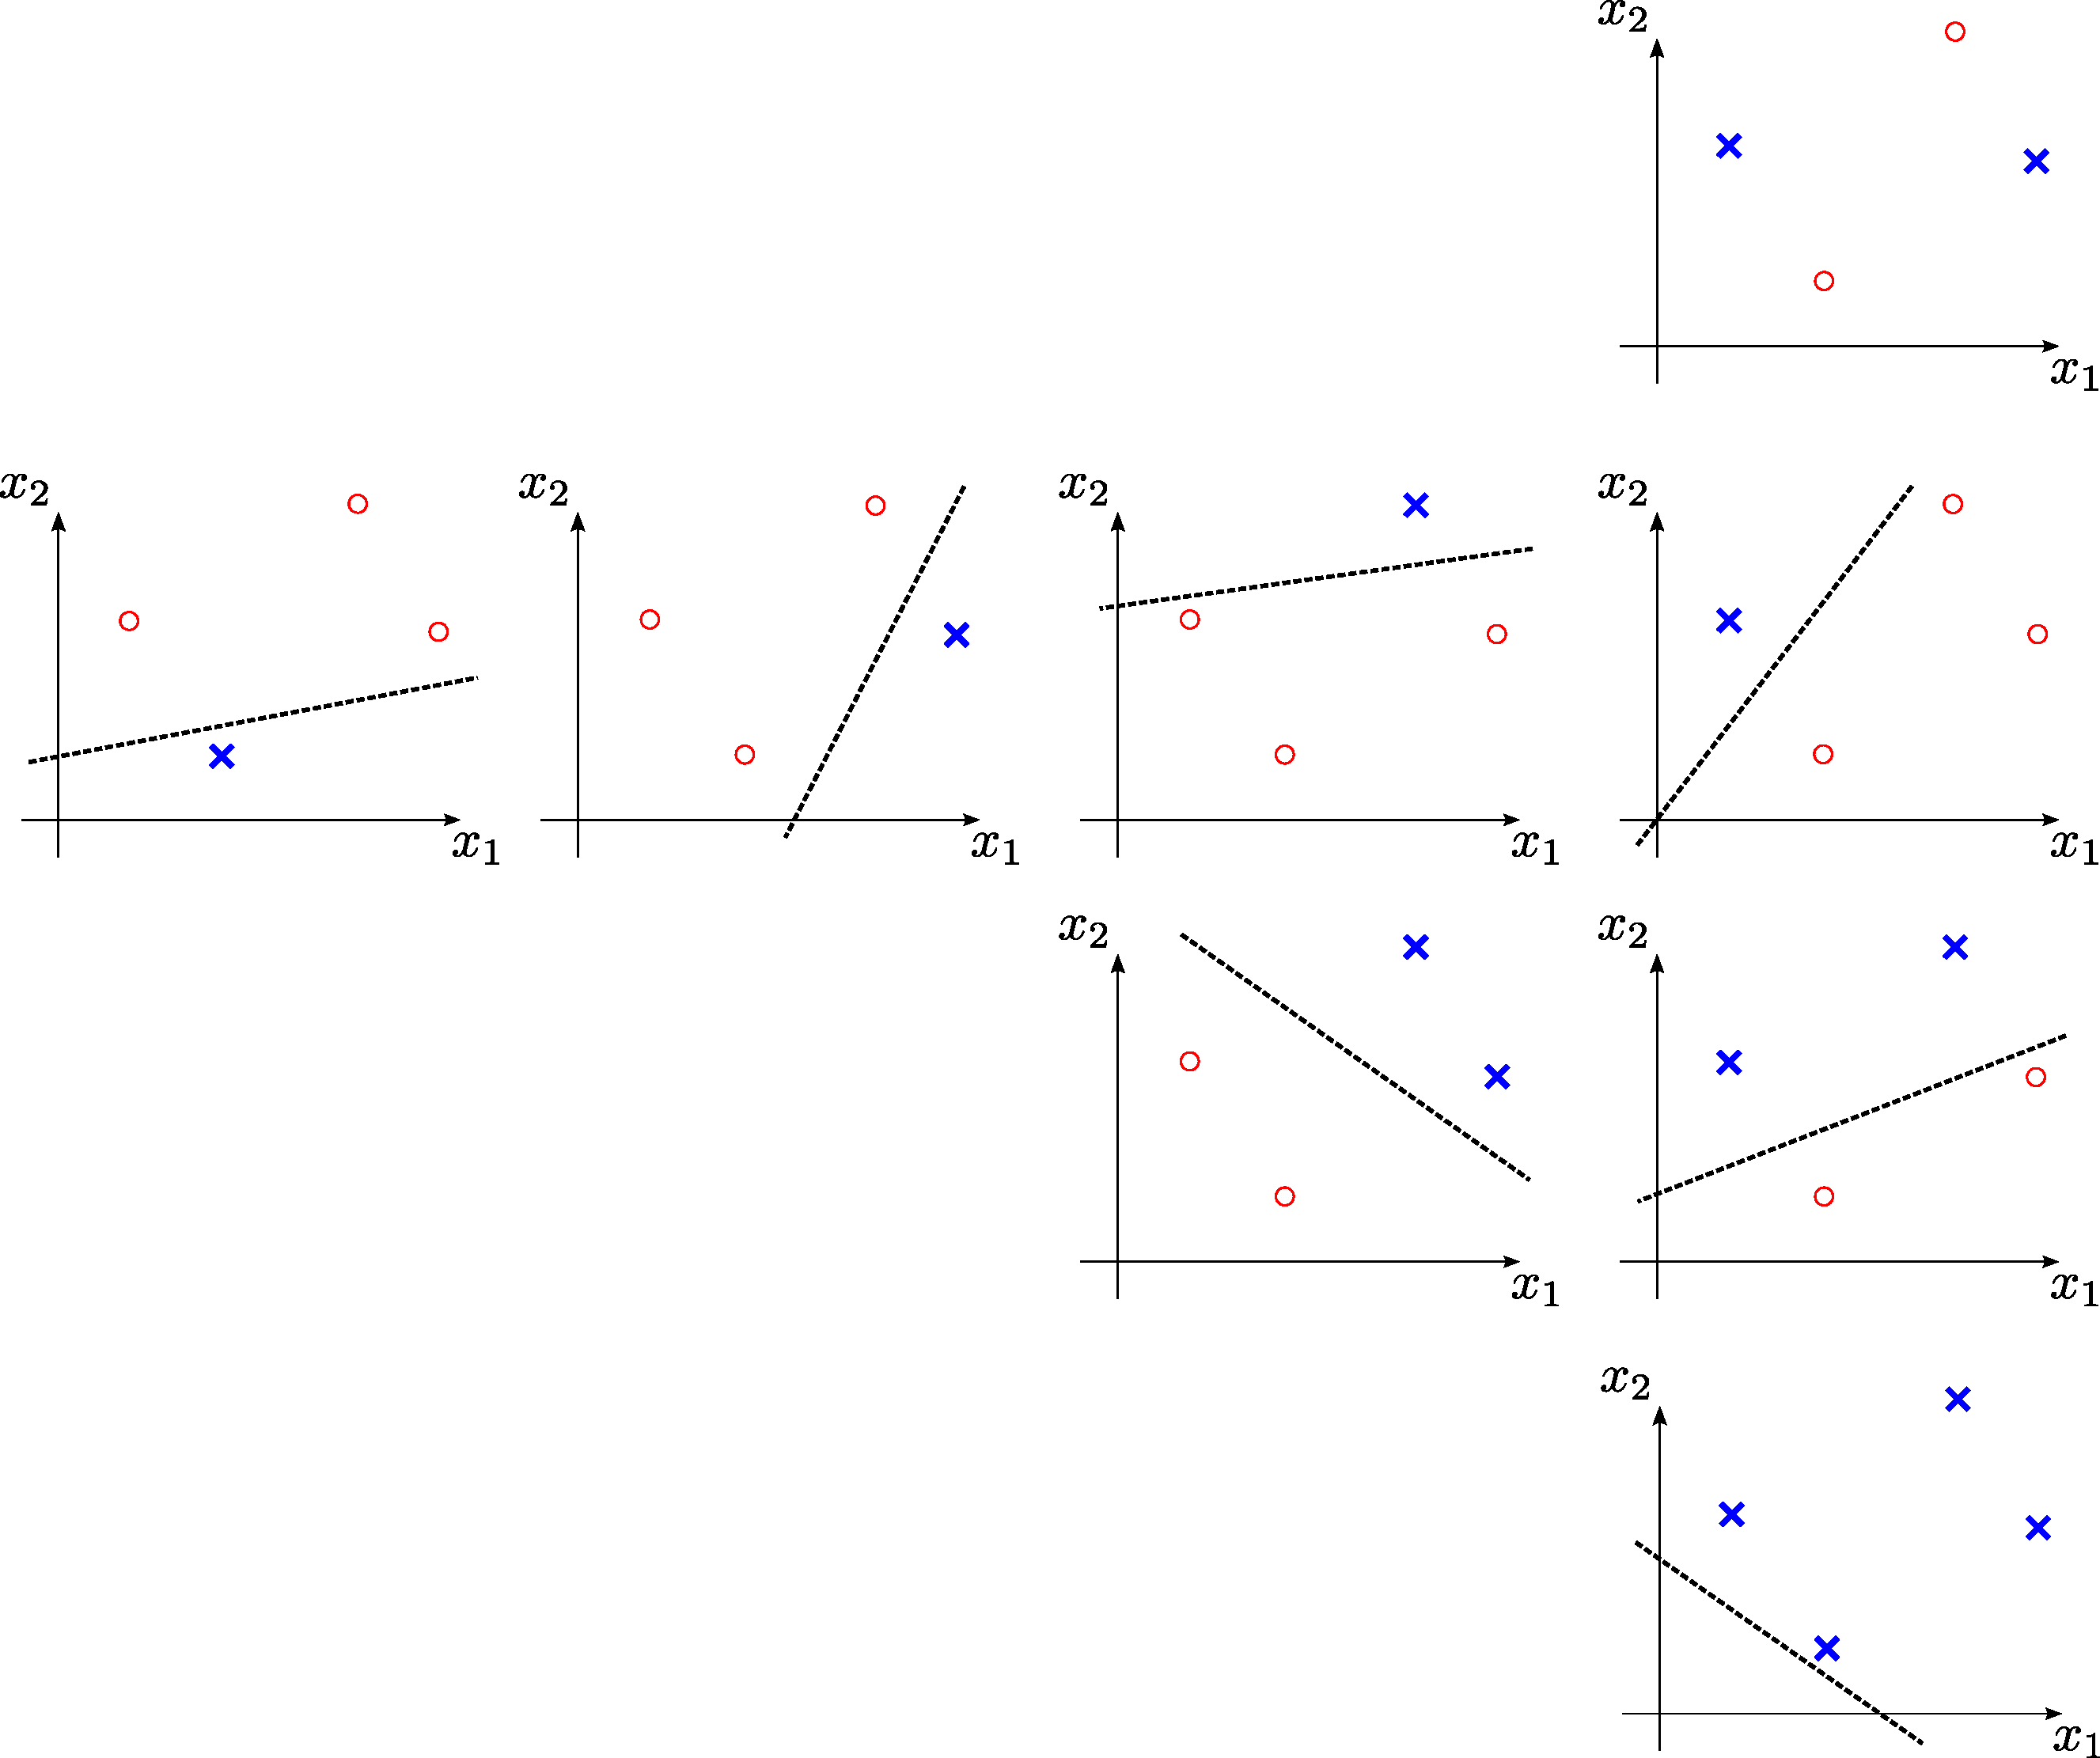
\includegraphics[width=0.85\textwidth]{img/linearly_sep}
            \mode<article>{
			\caption{Classifying 4 points in 2D. Multiply by 2 (reverse classification) to get all possible $2^4 = 16$ configurations. 2 of those configurations, the XOR- (top-right) and XNOR-like configurations are not linearly separable.}
            }
		\end{figure}
\end{frame}

\begin{frame}\frametitle{Calculate the number of configurations that are linearly separable}

Calculate the number of linearly separable assignments:

\begin{equation}
	\tilde C_{(p,N)} := 2 \sum_{k=0}^{N} 
	\underbrace{
	\left( \begin{array}{c}
	p-1\\
	k
	\end{array}\right)
	}_{\substack{\text{Binomial}\\ \text{coefficient}}}
\end{equation}

The Binomial coefficient\footnote{
See \href{https://en.wikipedia.org/wiki/Pascal\%27s_triangle}{Pascal's triangle} for a fun way on how to manually compute the coefficient.
} 
(``$n$ choose $k$'') 
is defined as:

\begin{equation}
\left(n \atop k \right) = \frac{n!}{k! (n-k)!}
\end{equation}

for $n,k \in \N_0$ with $n \ge k \ge 0$

\end{frame}

%\begin{frame}\frametitle{The Binomial coefficient}
\mode<article>{
The Binomial coefficient represents the coefficient associated with the $y^k$ term in the polynomial expansion $(1+y)^n$.

Consider the following example\footnote{
The example is taken from the Wikipedia article on \href{https://en.wikipedia.org/wiki/Binomial_coefficient}{Binomial coefficient}
} of using polynomial expansion for calculating the fourth power of $(1+y)$:

\begin{align}
(1+y)^4 &= 
\left({4 \atop 0}\right) y^0 +
\left({4 \atop 1}\right) y^1 +
{\color{blue}\left({4 \atop 2}\right) y^2} +
\left({4 \atop 3}\right) y^3 +
\left({4 \atop 4}\right) y^4\\
&= 1 + 4y + {\color{blue}6y^2} + 4y^3 + y^4
\label{eq:polyexpansion}
\end{align}

The binomial coefficient $\left({4 \atop 2}\right) = \frac{4!}{2!(4-2)!} = 6$. ${\color{blue}6}$ matches the coefficient in front of the ${\color{blue}y^2}$ term in the expansion\notesonly{ in \eqref{eq:polyexpansion}}.
}
%\end{frame}

\begin{frame}\frametitle{Calculating the number of separable configurations?}

\begin{equation*}
	\tilde C_{(p,N)} := 2 \sum_{k=0}^{N} \left( \begin{array}{c}
	p-1\\
	k
	\end{array}\right)
	\label{eq:cwithbias}
\end{equation*}

Using our example with $p=4$ and $N=2$:
\begin{align}
	\tilde C_{(4,2)} &= 2 \sum_{k=0}^{2} \left( \begin{array}{c}
	4-1\\
	k
	\end{array}\right)\\
	&= 2 \,
	\bigg\lbrack
	%\underbrace{
	\left({4-1 \atop {\color{black}0}}\right)
	%}_{\substack{\text{all positive}\\ \text{{\color{red}none} negative}}}
	+
	%\underbrace{
	\left({4-1 \atop {\color{black}1}}\right)
	%}_{\substack{\text{{\color{red}1} out of p}\\ \text{negative}}}
	+
	%\underbrace{
	\left({4-1 \atop {\color{black}2}}\right)
	%}_{\substack{\text{{\color{red}2} out of p}\\ \text{negative}}}
	\bigg\rbrack\\
	&= 2 \, \Big\lbrack
	1 + 3 + 3
	\Big\rbrack\\
	&= 14
\end{align}


\end{frame}

\begin{frame}

\mode<presentation>{

\begin{equation*}
	\tilde C_{(p,N)} := 2 \sum_{k=0}^{N} \left( \begin{array}{c}
	p-1\\
	k
	\end{array}\right)
\end{equation*}
}

\textbf{But} this looks slightly different from what is in the lecture. In the lecture it looked like this:

\begin{equation}
	C_{(p,N)} := 2 \sum_{k=0}^{N-1} \left( \begin{array}{c}
	p-1\\
	k
	\end{array}\right)
	\label{eq:cnobias}
\end{equation}

\question{Why does the sum for $\tilde C_{(p,N)}$ run to $N$ instead of $N-1$?}\\

\mode<article>{
-The difference between $\tilde C_{(p,N)}$ from \eqref{eq:cwithbias} and $C_{(p,N)}$ from \eqref{eq:cnobias} look different is due to the fact that $\tilde C_{(p,N)}$ computes the sum for $k=1,\ldots,N$ instead of stopping at $N-1$. This way the sum iterates over the degrees of freedom in a connectionis neuron which has a bias term. 
Choosing a connectionist neuron to separate the classes involves $N+1$ degrees of freedom because we add the bias term (the ability to translate the hyperplane).
Therefore, the reason betweenn the two definitions is the model choice and assuming that $C_{(p,N)}$ counts separability around the origin without the ability to shift the hyperplane.

-An alternative explanation to the difference between $\tilde C_{(p,N)}$ and $C_{(p,N)}$ is how to interpret $N$. The definition of $C_{(p,N)}$ treats $N$ as the parameters of the hyperplane. Therefore the bias is implicit.
If we assume that $N$ is the number of components in $\vec x$ and we need to prepend a bias term to it, we compute the number of separable configurations using $\tilde C_{(p,N)}$. 
It is important to understand that $\tilde C_{(p,N)}$ and $C_{(p,N)}$ effectively yield the same result when we feed each the appropriate arguments.
}
\end{frame}

\begin{frame}
Recursive formula for the binomial coefficient:
\begin{equation}
			\left( \begin{array}{c}
			n\\
			k
			\end{array}\right)+
			\left( \begin{array}{c}
			n\\
			k-1
			\end{array}\right)=
			\left( \begin{array}{c}
			n+1\\
			k
			\end{array}\right)
\end{equation}

Use the the recursive formula for the binomial coefficient to show that:

\begin{equation}
\tilde C_{(p,N)}+\tilde C_{(p,N-1)}=\tilde C_{(p+1,N)}
\label{eq:c_relation}
\end{equation}

The relevance of \notesonly{\eqref{eq:c_relation}}\slidesonly{ this} relationship becomes apparent when attempting to derive the VC dimension\notesonly{ (introduced in \sectionref{seq:dvc})} of a connectionist neuron.

\end{frame}

\begin{frame}
\mode<presentation>{
\only<1,2>{Show that}
\vspace{-5mm}
}

{
\begin{align}
\only<1,2>{
	\tilde C_{(p,N)} 
	\qquad + \quad \tilde C_{(p,N-1)} \;\;\quad
    &= \slidesonly{\qquad} \tilde C_{(p+1,N)}\qquad\\
    \notesonly{
	\intertext{Plugging in \eqref{eq:cwithbias} for each:}
	}
}
\only<1-4>{
    2 \sum_{k=0}^{N} \left(\kern-1ex \begin{array}{c}
	p-1\\
	k
	\end{array} \kern-1ex \right)
    +
    2 \sum_{k=0}^{N-1} \left(\kern-1ex \begin{array}{c}
	p-1\\
	k
	\end{array} \kern-1ex \right)
    &= 
    2 \sum_{k=0}^{N} \left(\kern-1ex \begin{array}{c}
	p+1-1\\
	k
	\end{array} \kern-1ex \right)\only<4->{\slidesonly{\\[-20mm]}
}
}
\only<2-4>{
	\intertext{Simplify the LHS by modifying the sums \notesonly{such that}\slidesonly{s.t.} they share the same limits.}
}
\only<2-5>{
	{\color{magenta}
    2 \left(\kern-1ex \begin{array}{c}
	p-1\\
	0
	\end{array}\kern-1ex\right)}
    +
    2 \sum_{k={\color{magenta}\cancel{0}1}}^{N} \left(\kern-1ex \begin{array}{c}
	p-1\\
	k
	\end{array} \kern-1ex \right)
    +
    2 \sum_{k=0}^{N{\only<3,4>{\color{red}}-1}} \left(\kern-1ex \begin{array}{c}
	p-1\\
	k
	\end{array}\kern-1ex\right)
    &= 
    2 \sum_{k=0}^{N} \left(\begin{array}{c}
	p\\k
	\end{array}\right)\\
}
\only<3-5>{
	{\color{magenta}
    2 \left(\kern-1ex \begin{array}{c}
	p-1\\ 0
	\end{array} \kern-1ex \right)}
    + 2~
    {\color{blue}
    \sum_{k=1}^{N}
    }\left(\kern-1ex \begin{array}{c}
	p-1\\ k
	\end{array} \kern-1ex \right)
    + 2~
    {\color{blue}
    \sum_{k=1}^{N}
    } \left(\kern-1ex \begin{array}{c}
	p-1\\ k{\color{red}-1}
	\end{array} \kern-1ex \right)
    &=\\
    %2 \sum_{k=0}^{N} \left( \begin{array}{c}
	%p\\ k
	%\end{array}\right)
	%\\
}
\only<4-5>{
	{\color{magenta}
    2 \left(\kern-1ex \begin{array}{c}
	p-1\\ 0
	\end{array} \kern-1ex \right)}
    + 2~
    {\color{blue}
    \sum_{k=1}^{N}
    }
    \bigg \lbrack \underbrace{
    \left(
    \begin{array}{c}
	p-1\\ k
	\end{array}\right)
    +\left(
    \begin{array}{c} 
	p-1\\ k-1
	\end{array}\right)
    }_{=\left(
    \begin{array}{c} 
	p\\ k
	\end{array}\right)\text{ (using the recursive property)}}
    \bigg 
    \rbrack
    &=\\
}
\only<5,6>{
    {\color{magenta}2} \underbrace{
		{\color{magenta}
		\left(\kern-1ex \begin{array}{c}
		p-1\\ 0
		\end{array} \kern-1ex \right)}
	}_{=1=\left( \begin{array}{c}
	p\\ 0
	\end{array}\right)}
    +
    2~{\color{blue}\sum_{k=1}^{N}}\left( \begin{array}{c}
	p\\ k
	\end{array}\right)
    &= 2 \sum_{k=0}^{N}
    \left( \begin{array}{c}
	p\\ k
	\end{array}\right)\\
\intertext{$\left({p \atop 0}\right)$ can now be \textcolor{red}{absorbed} into the sum.}
2 \sum_{k={\color{red}0}}^{N}
    \left( \begin{array}{c}
	p\\ k
	\end{array}\right)
    &=
2 \sum_{k=0}^{N}
    \left( \begin{array}{c}
	p\\ k
	\end{array}\right)
	}
\end{align}
}
\mode<presentation>{
\only<6>{
\begin{equation*}
\tilde C_{(p,N)}+\tilde C_{(p,N-1)}=\tilde C_{(p+1,N)}
\end{equation*}
}
}

\end{frame}

\mode*

\clearpage

\mode<all>
\section{Convergence of Empirical Risk Minimization (ERM)}

\mode<presentation>{
\begin{frame} 
    \begin{center} \huge
        \secname
    \end{center}
\end{frame}
}

\begin{frame}\frametitle{The learning problem}
    \mode<article>{
    \begin{center}
		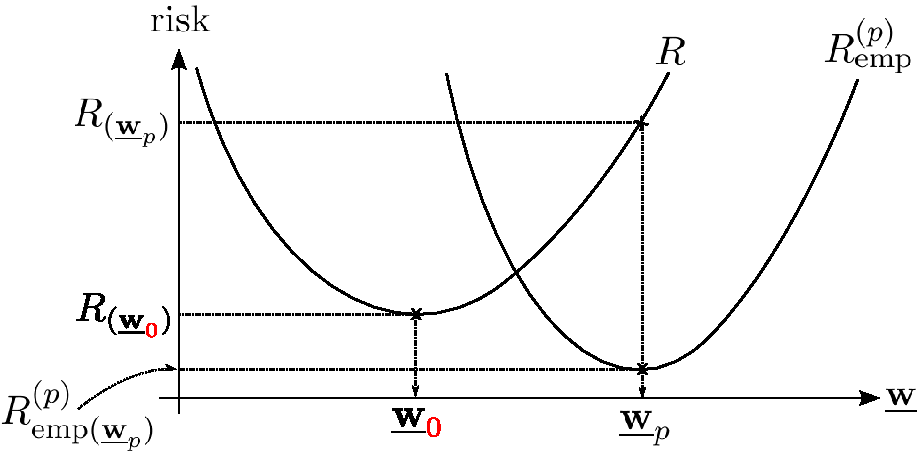
\includegraphics[height=4cm]{img/section2_fig1_highlight}
		\captionof{figure}{Comparing risk with empirical risk using a finite set with $p$ points.}
        \label{fig:riskvsemprisk}
	\end{center}
    }
    \mode<presentation>{
		\placeimage{8}{3}{img/section2_fig1_highlight}{width=6cm}
    }
    \underline{Setting}:\\
    
	\begin{itemize}
		\item {\footnotesize samples are drawn \iid~from $P(\vec x, y_T)$\\[1mm]
			 $\quad \leadsto \quad$ $\vec w$ are random variables}
        \item $R_{emp}\,\corresponds\,E^{T}_{[\vec w]}$ \notesonly{with $R_{(\vec w_{p})} \leftarrow \min R_{emp}$: the empirical risk obtained from training the model using a finite set with $p$ points, and}
        \item \hspace{6mm}$R\,\corresponds\,E^{G}_{[\vec w]}$\notesonly{with $R_{(\vec w_{\color{red}0})} \leftarrow \min R$}\\
        \slidesonly{\vspace{5mm}}
        
        Recall that
        \begin{eqnarray} \hspace{5mm} 
			E_{[\vec{w}]}^G 
			&=& \text{probability of misclassification} \\[-1mm]
			&=& \int P_{(y_T, \vec{x})} \,
				e_{(y_T, \vec{x};\vec{w})} \, 
				d \vec{x} \, d y_T \;\;\eqexcl\;\; \min_{\vec w}
		\end{eqnarray}
        
        \notesonly{
        Therefore, $R_{[\vec w_0]}$ represents the risk value obtained from training the model using infinitely many points.
        }
        (Don't treat the ${\color{red}_0}$ as zero data points but rather as ``minimal'' risk)
	\end{itemize}
\end{frame}

% -----------------------------------------------------------------------------
\definecolor{question1}{rgb}{0,0,1}
\definecolor{question2}{rgb}{0,0.5,0}
\subsection{The key questions of Statistical Learning Theory}
\begin{frame}\frametitle{\subsecname}
	\only<1>{
	\begin{center} 
	\slidesonly{
		\includegraphics<1>[height=4cm]{img/section2_fig1_question1}
		}
	\end{center}
		\begin{enumerate}
		\item When does inductive learning through ERM work?
		\begin{itemize}
		%\slidesonly{
		%\vspace{-5mm}
		%\item {\footnotesize $p$ samples are drawn \iid~from $P(\vec x, y_T)$\\[1mm]
			 %$\quad \leadsto \quad$ $\vec w$ are random variables}
			 %}
		\item 
			\vspace{1mm}
			%\iitem
			{$R_{\text{emp}(\vec w_p)}$ 
				should reflect the true optimal risk $R_{(\vec w_0)}$ 
				in the limit $p \to \infty$:}
			\vspace{1mm}
			\begin{equation}
				\lim_{p \rightarrow \infty} P \Big\{ 
						{\color{question1} \big| R_{(\vec{w}_p)}
						- R_{(\vec{w}_0)} \big| }
					\geq \eta \Big\} \;\;=\;\; 0 \,,
					\quad\text{ for all }\quad \eta > 0 \,.
				\label{eq:absdeltaconvergence0}
			\end{equation}
		\end{itemize}
		\end{enumerate}
		}
\only<2>{
%\end{frame}

%\begin{frame}
\label{sec:convergence_erm}
\frametitle{Understanding what $P\big\{ 
	{\color{question1}
		\big|R_{(\vec w_p)} - R_{(\vec w_0)}\big| 
	} \geq \eta \big\}$ represents
}

			%And this difference becoming smaller and smaller as we feed more points into the model. That is:
			%\begin{equation}
				%\lim_{p \to \infty} P\bigg\{ 
					%{
						%\Big|R_{[\vec w_p]} - R_{[\vec w_0]}\Big| 
					%}
				%\geq \eta \bigg\}\;\;=\;\; 0 \,, \quad \forall \eta > 0
				%\label{eq:erm_converges_zero}
			%\end{equation}
\mode<presentation>{
	\placeimage{8}{5}{img/section2_fig1_question1_many_p}{width=6cm}
}
\begin{figure}
	\mode<article>{ \centering }
	\mode<presentation>{ \raggedright \vspace{-2mm}}
	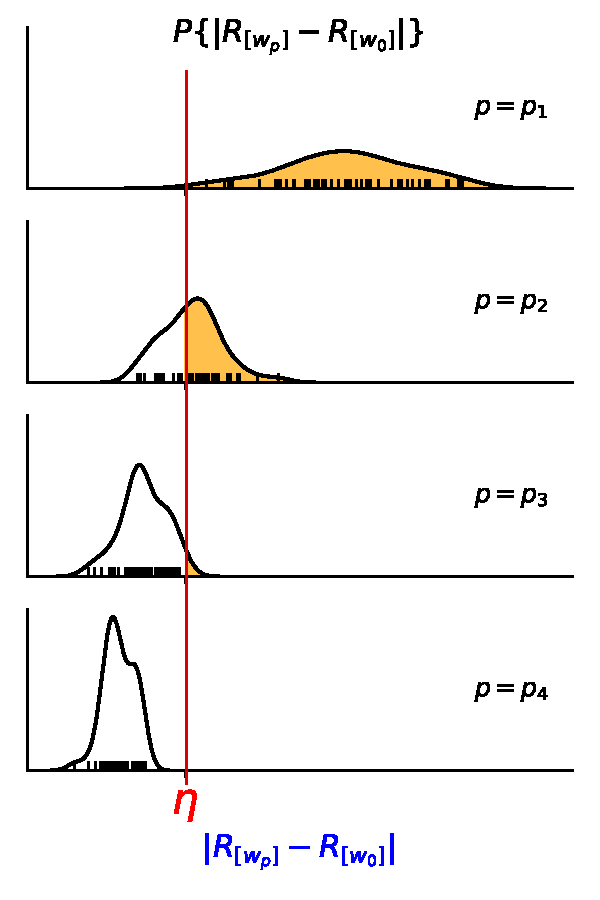
\includegraphics[height=\slidesonly{6.7cm}{\notesonly{8cm}}]{img/PdeltaReta}
	\caption{Distribution of absolute risk differences for larger number of training points $p_{1} < p_{2} < p_{3} < p_{4}$}
	\label{fig:PdeltaReta}
\end{figure}
}
\end{frame}
	
\mode<article>{			
			Understanding \figref{fig:riskvsemprisk} and
			what \eqref{eq:absdeltaconvergence0} represents:
				
			\begin{itemize}
			\item We expect the model trained on $p$ points to have  some error $R_{\text{emp}}$ that is minimal for some $\vec w_p$ at which the empirical error is $R_{\text{emp}(\vec w_p)}$.
			\item Estimating the generalization performance for the solution $\vec w_p$ on a hold-out set yields a risk value of $R_{(\vec w_p)}$. We expect it to be higher than the optimal risk $R_{(\vec w_0)}$. We therefore measure the absolute difference between both:
			\begin{equation}
			{\color{question1}
			\big| R_{(\vec{w}_p)}
						- R_{(\vec{w}_0)} \big|
						}
			\end{equation}
			\item Training the model with a different set of $p$ points (the size of the training set is kept at $p$) may yield a different minimum for $R_{\text{emp}(\vec w_p)}$ with a corresponding generalization performance $R_{(\vec w_p)}$ and consequently a different absolute difference ${\color{question1}
			\big| R_{(\vec{w}_p)}
						- R_{(\vec{w}_0)} \big|
						}$
			\item Training many models while keeping $p$ fixed will yield many values for the absolute difference ${\color{question1}
			\big| R_{(\vec{w}_p)}
						- R_{(\vec{w}_0)} \big|
						}$
			\item Measuring the absolute difference between every $R_{(\vec w_p)}$ we obtained and $R_{(\vec w_0)}$ will lead to ``difference values'' that follow some distribution $P\big\{ 
					{\color{question1}
						\big|R_{(\vec w_p)} - R_{(\vec w_0)}\big| 
					}
				\geq \eta \big\}$
			\item We measure the probability of the absolute difference being equal or exceeding some nonnegative value $\eta$:
			\begin{equation}
			P\big\{ 
					{\color{question1}
						\big|R_{(\vec w_p)} - R_{(\vec w_0)}\big| 
					}
				\geq \eta \big\}\,, \quad \forall \eta > 0
			\end{equation}
			This is the same as asking: How often does training with $p$ points yield a difference in risk above some value.
			\item Now we repeat the training of these models but using a larger value for $p$.\\
			
			What the theory tells you here is that as you increase $p$ and keeping $\eta$ fixed:
			\begin{itemize}
				\item The $R_{(\vec w_p)}$ of the models will improve and get smaller.
				\item The absolute differences ${\color{question1}\big|R_{(\vec w_p)} - R_{(\vec w_0)}\big|}$ will become smaller and smaller,
				\item As depicted by \figref{fig:PdeltaReta}, the distribution of these differences will shift to the left of $\eta$.
				\item Less and less models will score differences $\ge \eta$
				\item Eventually, for some large $p$, the $R_{(\vec w_p)}$ of the models will be so good that the probability of finding a model that has a risk difference of $\eta$ or higher (worse performance) will vanish. And this is what \eqref{eq:absdeltaconvergence0} describes.
			\end{itemize}
			\end{itemize}
			%\begin{equation}
				%\lim_{p \to \infty} P\bigg\{ 
					%{\color{question1}
						%\Big|R_{(\vec w_p)} - R_{(\vec w_0)}\Big| 
					%}
				%\geq \eta \bigg\}\;\;=\;\; 0 \,, \quad \forall \eta > 0
				%\label{eq:risktozero}
			%\end{equation}
			
			\textbf{But} Our dataset is never going to be infinitely large. Therefore a more realistic formulation for the convergence of ERM would be that the probability will fall below some value $\epsilon$ which gives rise to the next key question from Statistical Learning Theory:
            
            \begin{enumerate}
            \item[2] How strongly does $R_{(\vec{w}_p)}$ differ 
				from $R_{(\vec{w}_0)}$ for  \textbf{finite} samples?
				\vspace{1mm}
				\iitem{For a given confidence $\epsilon$, find $\eta$ such that}
				\vspace{1mm}
                
                \begin{equation}
					P \Big\{ {\color{question1} 
							\big| R_{(\vec{w}_p)} - R_{(\vec{w}_0)} \big| 
						} \geq \eta \Big\} \;\;<\;\; \epsilon \,.
						\label{eq:convergenceeps}
				\end{equation}
            \end{enumerate}
            
				
			Furthermore, recalling what we've learned about the bias-variance tradeoff, the solution that minimizes $R_{\text{emp}}$ might not be a favorable solution. We therefore extend the comparison of the curves $R_{\text{emp}}$ with $R$ to include other solutions that do not necessarily minimize the empirical risk $R_{\text{emp}}$ (i.e. training error). This leads to further modifying our formulation of the convergence from \eqref{eq:convergenceeps} in order to formulate the next key question from Statistical Learning Theory:
            
            \begin{enumerate}
            \item[3] Do training errors $R_{\text{emp}(\vec w)}$ 
				reflect generalization performance $R_{(\vec w)}$?
				\vspace{1mm}
				\iitem{\footnotesize Avoid overfitting for finite samples,
				i.e.~given confidence $\epsilon$, find $\eta$ such that: 
					%i.e.~$R_{(\vec w)} \approx R_{\mathrm{emp}(\vec w)}$:
				}
                
				\begin{equation}
					P \Big\{ {\color{question2}
							\big| R_{(\vec w)} - R_{\mathrm{emp}(\vec w)} \big|
						} > \eta \Big\} \;\;<\;\; \epsilon \,, 
						\qquad \forall \vec w \in \Lambda \,.
						\label{eq:convergenceepsgeneral}
				\end{equation}
            \end{enumerate}
			
			The key difference between \eqref{eq:convergenceeps} and \eqref{eq:convergenceepsgeneral} is that the latter is no longer restricted to the solutions $\vec w_p$ at which the empirical risk is minimal but may include solutions $\vec w$ that can potentially generalize better.
}
\mode<presentation>
{
\begin{frame}\frametitle{\subsecname}
	\begin{center} 
	\slidesonly{
		\includegraphics<1>[height=4cm]{img/section2_fig1_question1}
		}
		\begin{center}
			\includegraphics<2->[height=4cm]{img/section2_fig1_question2_lessw} 
			\mode<article>{
			\captionof{figure}{
			Measuring the difference between empirical risk obtained from a finite site of $p$ points with risk obtained using infinitely many points.
			}
			\label{fig:randremp}
			} 
		\end{center}
	\end{center}
	
	\only<1>{
		\begin{enumerate} \setcounter{enumi}{1}
			\item How strongly does $R_{(\vec{w}_p)}$ differ 
				from $R_{(\vec{w}_0)}$ for  \textbf{finite} samples?
				\vspace{1mm}
				\iitem{For a given confidence $\epsilon$, find $\eta$ such that}
				\vspace{1mm}
				\begin{equation}
					P \Big\{ {\color{question1} 
							\big| R_{(\vec{w}_p)} - R_{(\vec{w}_0)} \big| 
						} \geq \eta \Big\} \;\;<\;\; \epsilon \,.
						%\label{eq:convergenceeps}
				\end{equation}
		\end{enumerate}
	} \only<2>{
		\begin{enumerate} \setcounter{enumi}{2}
			\item Do training errors $R_{\text{emp}(\vec w)}$ 
				reflect generalization performance $R_{(\vec w)}$?
				\vspace{1mm}
				\iitem{\footnotesize Avoid overfitting for finite samples,
				i.e.~given confidence $\epsilon$, find $\eta$ such that: 
					%i.e.~$R_{(\vec w)} \approx R_{\mathrm{emp}(\vec w)}$:
				}
				\vspace{1mm}
				\begin{equation}
					P \Big\{ {\color{question2}
							\big| R_{(\vec w)} - R_{\mathrm{emp}(\vec w)} \big|
						} > \eta \Big\} \;\;<\;\; \epsilon \,, 
						\qquad \forall \vec w \in \Lambda \,.
						%\label{eq:convergenceepsgeneral}
				\end{equation}
                where $\Lambda$ is the model class (e.g. connectionist neuron)
		\end{enumerate}
	}
\end{frame}
}

\mode*

\clearpage

\mode<all>
\section{The Vapnik-Chervonenkis (VC) dimension}\label{seq:dvc}

\mode<presentation>{
\begin{frame} 
    \begin{center} \huge
        \secname
    \end{center}
\end{frame}
}

\begin{frame}\frametitle{Shattering $p$ points}

\question{Can a perceptron classify any 3 points in 2D?}\\

\visible<2>{
- Yes, as long as they're not colinear.%\textbf{see blackboard...}
}

\question{Can a perceptron classify any 4 points in 2D?}\\

\visible<2>{
- No, it cannot.%\textbf{see blackboard...}
}

\end{frame}

\begin{frame}\frametitle{Shattering $p$ points}

\mode<presentation>{
	\only<1>{
		\placeimage{12.5}{7.5}{img/shatter_arrangement_2_points}{width=2.5cm}
	}
	\only<2>{
		\placeimage{12.5}{7.5}{img/shatter_arrangement_2_points_model}{width=2.5cm}
	}
	\only<3>{
		\placeimage{12.5}{7.5}{img/shatter_arrangement_2_points_model_label}{width=2.5cm}
	}
	\only<4,5>{
		\placeimage{12.5}{7.5}{img/shatter_arrangement_2_points_model_label_decisions}{width=2.5cm}
	}
	\only<6>{
		\placeimage{12.5}{7.5}{img/shatter_arrangement_2_points_model_label_shatter}{width=2.5cm}
	}
}

\begin{enumerate}
\item Generate a dataset of $p$ points in $N$ dimensions and place them in some arrangement.
\pause
\item Decide on a model class $\Lambda$ (e.g. connectionist neuron with bias)
\pause
\item For each possible binary label configuration (total: $2^p$) $\{y_T^{(\alpha)}\}_{\alpha=1}^p$ do
	\begin{itemize}
	\item[] Train the parameters $\vec w$ of a model from the set $\Lambda$.
	\item[] Generate binary predictions $\{y^{(\alpha)}(\vec x^{(\alpha)}; \vec w)\}_{\alpha=1}^p$
	\item[] Measure the error $E^T_{[\vec w]}$
	\item[] If $E^T_{[\vec w]} = 0$ keep the model, otherwise, discard it. 
	\end{itemize}
\pause
\item Count how many models you've kept.\\
\pause
\item[] If you were able to keep a model with $E^T_{[\vec w]} = 0$ for each of the $2^p$ possible label configurations,\\
then the model class $\Lambda$ with that number of tunable parameters in $\vec w$ \emph{shatters} a dataset of $p$ points in $N$ dimensions.
\end{enumerate}

\end{frame}

\begin{frame}\frametitle{Shattering a dataset}

\textbf{Important}:\\

Shattering requires finding \underline{at least one arrangement} of the $p$ points for which the model can be fitted to all $2^p$ label configurations.

\pause 

\svspace{10mm}

\begin{center}
\begin{minipage}{0.45\textwidth}
\begin{center}
	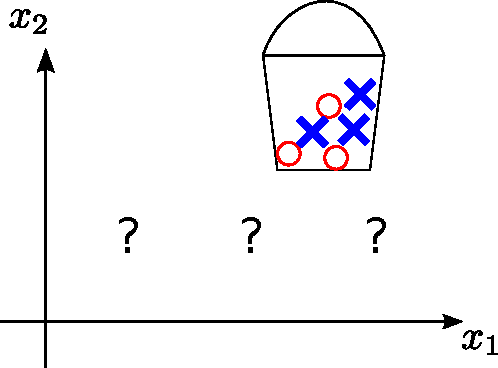
\includegraphics[width=0.7\textwidth]{img/shatter_arrangement_1}
	\notesonly{
	\captionof{figure}{A perceptron cannot always separate this arrangement.}
	}
\end{center}
\end{minipage}
\begin{minipage}{0.45\textwidth}
\begin{center}
	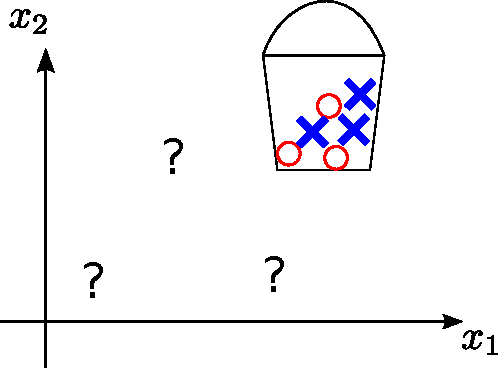
\includegraphics[width=0.7\textwidth]{img/shatter_arrangement_2}
	\notesonly{
	\captionof{figure}{A perceptron can always separate this arrangement.}
	}
\end{center}
\end{minipage}
	\notesonly{
	\captionof{figure}{An arrangement of 3 points in 2D.}
	}
\end{center}

\mode<article>{
It does not have to be able to for all possible arrangements (placements) of the $p$ points.
If there exists at least \textbf{one} dataset for which it can perfectly predict all label configurations, then the model shatters this.
}
\end{frame}

\begin{frame}\frametitle{\secname}


\mode<presentation>{
\begin{center}
	\includegraphics<1>[width=0.4\textwidth]{img/meme_vc_notdim}
\end{center}
}

\only<1>{
$\dvc$ is not actually a dimension but a single number \emph{capacity measure} 
of a model class that is parameterized by $\vec w$.\slidesonly{\\[5mm]}\notesonly{\\}
}

\underline{Definition}:\\

\only<1>{
$\dvc :=$ \underline{maximal number of data points $p$} that a model can \emph{shatter}.\\

}
\only<2>{
In other words, The VC dimension is the largest \# of points  
$p$ for which there exist at least one dataset  
$\vec X = \left(\vec x^{(1)}, \ldots, \vec x^{(p)}\right)^\top $ for which all  
$2^p$ label configurations can be solved with zero error.\\

}
\only<3>{
In more words: $\dvc$ is the \underline{maximal number of data points $p$} for which \emph{all} possible label configurations $\{y_{T}^{(\alpha)} \in \{-1,1\}\}_{\alpha=1}^{p}$ can be perfectly trained (i.e. $E^{T}_{[\vec w]} = R_{\text{emp}[\vec w]} = 0$) by tuning the model parameters $\vec w$.
If (at least) one dataset $\{(\vec x^{(\alpha)}, y_{T}^{(\alpha)})\}_{\alpha=1}^{p}$ with $p$ points exists such that the model can be tuned to perfectly classify any label configuration for that dataset, then the $\dvc$ for this model class is $p$.
}

\end{frame}

\begin{frame}

\mode<presentation>{
\begin{center}
\begin{minipage}{0.45\textwidth}
\begin{center}
	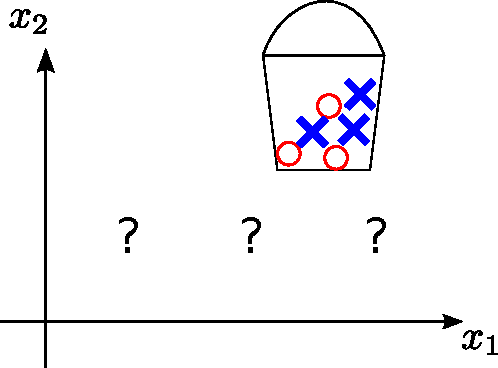
\includegraphics[width=0.7\textwidth]{img/shatter_arrangement_1}
	\notesonly{
	\captionof{figure}{A perceptron cannot always separate this arrangement.}
	}
\end{center}
\end{minipage}
\begin{minipage}{0.45\textwidth}
\begin{center}
	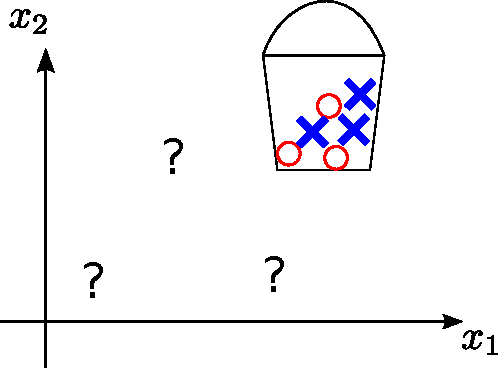
\includegraphics[width=0.7\textwidth]{img/shatter_arrangement_2}
	\notesonly{
	\captionof{figure}{A perceptron can always separate this arrangement.}
	}
\end{center}
\end{minipage}
	\notesonly{
	\captionof{figure}{An arrangement of 3 points in 2D.}
	}
\end{center}
}

\question{What was the $\dvc$ for our model in the previous example?}

\end{frame}

\begin{frame}

\underline{Examples}:

\begin{align}
&{\dvc}^{\text{perceptron}} &\kern-12ex=\;\;& N+1 = \text{\#params}\\
&{\dvc}^{\text{MLP}} &\kern-12ex=\;\;& \mathcal{O}(\text{\#params}^{2})\\
&{\dvc}^{1\text{NN}} &\kern-12ex=\;\;& \infty\\
&{\dvc}^{\text{sinusoid}} &\kern-12ex=\;\;& \infty
\end{align}

\begin{equation}
y^{\text{sinusoid}}(x;w) = \sign \big\lbrack \sin\left( w x \right) \big\rbrack    
\end{equation}

\pause

\question{How is ${\dvc}^{\text{sinusoid}} = \infty$? There's only 1 parameter!}

\mode<article>{
The parameters of the sinusoidal are amplitude, phase and frequency. A total of 3 parameters. Regardless of how many points there are, it is always possible to find values for the 3 parameters such that the sinusoidal goes through all $p$ points.
}
    
\end{frame}


\mode*

\clearpage

\mode<all>
\section{The growth function}

\mode<presentation>{
\begin{frame} 
    \begin{center} \huge
        \secname
    \end{center}
\end{frame}
}

\begin{frame}\frametitle{\secname~- What is it?}

The growth function is the measure of \emph{sample} complexity for a model class.\\[5mm]

It measures the complexity of the functions that can be fitted using a model from that model class (e.g. connectionist neuron).\\[5mm]

\emph{sample} complexity: \emph{how much can I do with $p$ points in $N$ dimensions?}\\[10mm]

It is closely related to the \emph{VC dimension}.

\end{frame}

\subsection{Defining the growth function}

\mode<presentation>{
\begin{frame} \frametitle{The growth function $G_{(p)}^\Lambda$}
	\begin{itemize}
		\item \textbf{data representation:} 
			$\vec{x} \in \mathbb{R}^N, \quad y_T \in \{-1,+1\}$ 
		\vspace{5mm}
		\item \textbf{model class:} 
			set $\Lambda$ of functions $y_{(\vec{x}; \vec{w})} \in \{-1,+1\}$
			
		\vspace{5mm}
		\item \textbf{binary label vector:} $\vec y_{(\vec{w})} = \Big( 
			y_{(\vec{x}^{(1)}, \vec{w})}, 
			y_{(\vec{x}^{(2)}, \vec{w})}, \ldots, 
			y_{(\vec{x}^{(p)}, \vec{w})} \Big)$
			\begin{itemize}	
				\item different classifiers can induce the 
					same label vector on the training set 
			\end{itemize}
			
		\vspace{5mm}
		\item \textbf{number of different vectors} $\vec y_{(\vec{w})}$ 
			induced by all $\vec w \in \Lambda$:
			\vspace{-2mm}
			\begin{equation}
				\tag{depends on $\Lambda$ and the sample}
				N_{(\vec{x}^{(1)}, \ldots, \vec{x}^{(p)})}^\Lambda 
				\;\;\leq 2^p 
			\end{equation}
	\end{itemize}
\end{frame}
}


\begin{frame} \frametitle{The growth function $G_{(p)}^\Lambda$}
	\begin{itemize}
		\item<1-> \textbf{data representation:} 
			$\vec{x} \in \mathbb{R}^N, \quad y_T \in \{-1,+1\}$ 
		\vspace{5mm}
		\item<1-> \textbf{model class:} 
			set $\Lambda$ of functions $y_{(\vec{x}; \vec{w})} \in \{-1,+1\}$
			
			Think of $\Lambda$ as a set of classifiers.
			The classifiers in this set come from the same model class (e.g. connectionist neurons with weights $\vec w$).
			Each classifier describes a different hyperplane (different $\vec w$) to separate the two classes in the data.
			
		\vspace{3mm}
		\item<2-> {\textbf{binary label vector}:} $\vec y_{(\vec{w})} = \Big( 
			y_{(\vec{x}^{(1)}, \vec{w})}, 
			y_{(\vec{x}^{(2)}, \vec{w})}, \ldots, 
			y_{(\vec{x}^{(p)}, \vec{w})} \Big)$
			\begin{itemize}	
				\item different classifiers can induce the 
					same label vector on the training set\notesonly{ (cf. \figref{fig:dichotomy_redundant})}
					
				%\begin{center}
					%\includegraphics<2>[width=0.25\textwidth]{img/dichotomy_redundant}
					%\notesonly{
					%\captionof{figure}{Different weight vectors that produce identical labelng of the points.}
					%}
					%\label{fig:dichotomy_redundant}
				%\end{center}
			\end{itemize}
			
			Each classifier in $\Lambda$ describes a different hyperplane.
            \mode<article>{
			Looking at the predictions each one produces for the $p$ points will produce some label vector $\vec y_{(\vec{w})}$ with $p$ elements. A prediction for every point.
			}
		\vspace{5mm}
		\item<3> \textbf{number} of different vectors $\vec y_{(\vec{w})}$ 
			induced by all $\vec w \in \Lambda$:
			\vspace{-2mm}
			\begin{equation}
				\tag{depends on $\Lambda$ and the sample}
				N_{(\vec{x}^{(1)}, \ldots, \vec{x}^{(p)})}^\Lambda 
				\;\;\leq 2^p 
			\end{equation}
	\end{itemize}
\end{frame}

\begin{frame}\frametitle{The growth function $G_{(p)}^\Lambda$ and $N^{\Lambda}$}
		Two hyperplanes can be different but still yield the same predictions.
		Example:\\
		\begin{figure}[h]
			\centering
			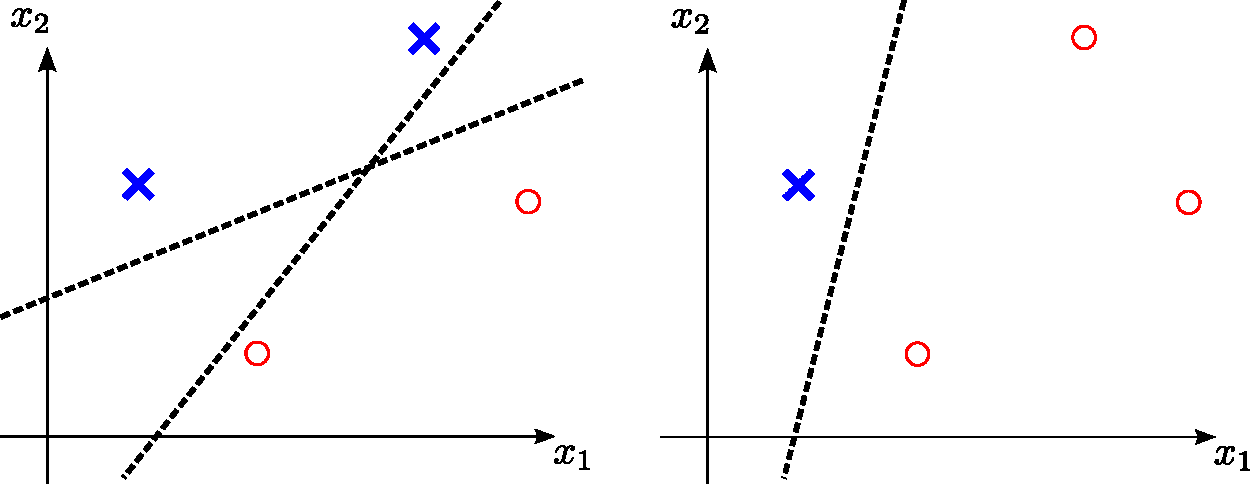
\includegraphics[width=0.6\textwidth]{img/uniquepredictions}
            \mode<article>{
			\caption{Different hyperplanes can lead to different but also to identical labeling of points}
            }
		\end{figure}
		\mode<article>{
		We are interested in the set of unique labeling vectors, more importantly, the size of this set. It tells us how many labeling configuration can be fitted by a model from the model class.
		The number of unique labeling vectors is 
		$N_{(\vec{x}^{(1)}, \ldots, \vec{x}^{(p)})}^\Lambda$
		
		Given that the total number of possible labeling configuration is $2^p$
		and that we cannot guarantee that the models from $\Lambda$ can be fitted to all of them, it follows:
		}
        \begin{equation}
            N_{(\vec{x}^{(1)}, \ldots, \vec{x}^{(p)})}^\Lambda
            \;\;\leq 2^p 
        \end{equation}
\end{frame}

\begin{frame}\frametitle{Defining the growth function $G_{(p)}^\Lambda$}

	\mode<article>{	
		There are various reasons for $N^\Lambda$ to fall below $2^p$. Maybe we didn't sample enough classifiers from $\Lambda$. To eliminate the effects of this ``sampling'' we look for the maximum value \emph{that can be obtained} (supremum) for $N^\Lambda$ and by looking at how this value behaves as a function of $p$ we arrive at the growth function:
		}
		
	%\begin{equation} 
			%G_{(p)}^\Lambda = \ln \underbrace{ \bigg( 
				%\sup_{\vec{x}^{(1)}, \ldots \vec{x}^{(p)}}
				%N_{(\vec{x}^{(1)}, \ldots, \vec{x}^{(p)})}^\Lambda \bigg) }_{
					%\text{worst case}}
	%\end{equation}
	\svspace{-3mm}
	\begin{equation}
	G_{(p)}^\Lambda = \ln \bigg( 
				\sup_{\vec{x}^{(1)}, \ldots \vec{x}^{(p)}}
				N_{(\vec{x}^{(1)}, \ldots, \vec{x}^{(p)})}^\Lambda \bigg) = \ln 2^p = p \ln 2
				\label{eq:growthln2}
	\end{equation}
	
    \notesonly{
	Before we proceed, we turn back to the convergence of ERM, specifically \eqref{eq:absdeltaconvergence0}:
    }
	\mode<presentation>{
    Recall:
    \svspace{-3mm}
				\begin{equation*}
				\lim_{p \to \infty} P\bigg\{ 
					{
						\Big|R_{[\vec w_p]} - R_{[\vec w_0]}\Big| 
					}
				\geq \eta \bigg\}\;\;=\;\; 0 \,, \quad \forall \eta > 0
			\end{equation*}
	}
	
	This convergence is equivalent to\footnote{\notesonly{We don't dig into how they are equivalent. }If interested, see Ch. 5.5 \citep{scholkopf2001learning} for a description of the approach and \citep{vapnik1999overview} for the detailed derivation.
	}:
	\begin{equation}
	\lim_{p \to \infty} G_{(p)}^\Lambda / p \eqexcl 0
	\end{equation}
	\mode<article>{
	In the case of $G_{(p)}^\Lambda = p \ln 2$ as per our definition of the growth function in \eqref{eq:growthln2}:
	}
	\begin{equation}
	\lim_{p \to \infty} \left( p \ln 2 \right ) / p = \ln 2 \ne 0
	\end{equation}
	
	\notesonly{
	There is no convergence to zero, regardless of $p$. According to Vapnik, this means that} the classifier's predictions become ambiguous and will likely fail to generalize.

\end{frame}

\begin{frame}{Complete ambiguity}
    The growth function does not tell us how many points we need to separate the two classes but how many points we need to exclude completely ambiguous predictions.\\
    
\end{frame}

\begin{frame}{Example with complete ambiguity}
    \notesonly{Example with complete ambiguity:\\}
    \mode<presentation>{
    
    Linear neuron, 2 points in 2D. We do not have access to the hyperplane $\vec w$. We only have access to the predictions made by the neuron:\\
    %\textbf{see blackboard\ldots}
    }
    
	\begin{center}
\slidesonly{
		\includegraphics<2>[width=0.3\textwidth]{img/dichotomy_ambiguous}
		\includegraphics<3>[width=0.3\textwidth]{img/dichotomy_ambiguous_new_point}
		}
		\includegraphics<4>[width=0.3\textwidth]{img/dichotomy_ambiguous_decision_boundaries}
		\notesonly{
		\captionof{figure}{Complete ambiguity over the label of a third point, when we only have the predictions of two points in 2D by a linear neuron.}
		}
	\end{center}
    
    \mode<article>{Any linear neuron can find a hyperplane to separate two specific points in 2-D space. It does not tell us anything about the neuron's ability to separate an additional 3rd test point in that same space. Therefore $p = 2$ is still ambiguous for the linear neuron.}
    
\end{frame}

\begin{frame}{Example with \textbf{non}complete ambiguity}
    \notesonly{An example with \textbf{no complete} ambiguity:\\}
    \mode<presentation>{
    
    Linear neuron, 3 points in 2D:\\
    %\textbf{see blackboard\ldots}
    }
    
	\begin{center}
\slidesonly{
		\includegraphics<1>[width=0.3\textwidth]{img/dichotomy_nonambiguous_new_point}
		}
		\includegraphics<2>[width=0.3\textwidth]{img/dichotomy_nonambiguous_decision_boundaries}
		\notesonly{
		\captionof{figure}{No complete ambiguity over the label of the third point in 2D.}
		}
	\end{center}
\end{frame}

\mode<article>{
\begin{frame}
However, for $p > \dvc$ the growth function behaves differently, namely
	\begin{equation}
		G^{\Lambda}_{(p)} \le \dvc (1+ ln \frac{p}{\dvc}
	\end{equation}
	
	In this case  $\lim_{p \to \infty} G_{(p)}^\Lambda$ converges to zero, and there is no more complete ambiguity. There is at least one region in feature space where all different classifiers from $\Lambda$ will agree on what class to assign to points in that region. There may still exist regions for which predictions will be ambiguous but the complete ambiguity is gone. The more points we add, the less likely a model will find a solution, but if it does, they will no longer be ambiguous.

%Maybe this provokes the question: Why is the plot even useful? If I change my model to something with a lower d_VC, all I'm doing is that I allow the linear part of G to stop and switch to the curvy part earlier. A lower d_VC means that the curvy part happens for less p where the p ln 2 is also lower. The range of ambiguous predictions becomes lower and I'm able to generalize with fewer training samples.
\end{frame}
}

\begin{frame}
	\begin{itemize}
		\item bound on growth function (Vapnik, 1998)
			\begin{equation}
				G_{(p)}^\Lambda
				\left \{ \begin{array}{ll}
					= p \ln 2 
					& \text{for } p \leq \dvc \\
					\leq \dvc \Big( 1 + \ln \frac{p}{\dvc} \Big) 
					& \text{for } p > \dvc
				\end{array} \right.
			\label{eq:growthpiecewise}
			\end{equation}

		\item Vapnik-Chernovenkis dimension $d_{VC}$: \\
			capacity measure of the model class
		%\itR the growth function is independent of a specific sample
		%\itR the growth function is bounded by a term logarithmic in $p$
		%\itR the growth rate depends on the model's VC-dimension $\dvc$ 
	\end{itemize}
\end{frame}

% -----------------------------------------------------------------------------
\begin{frame}\frametitle{The growth function $G_{(p)}^\Lambda$}
	\begin{center}
		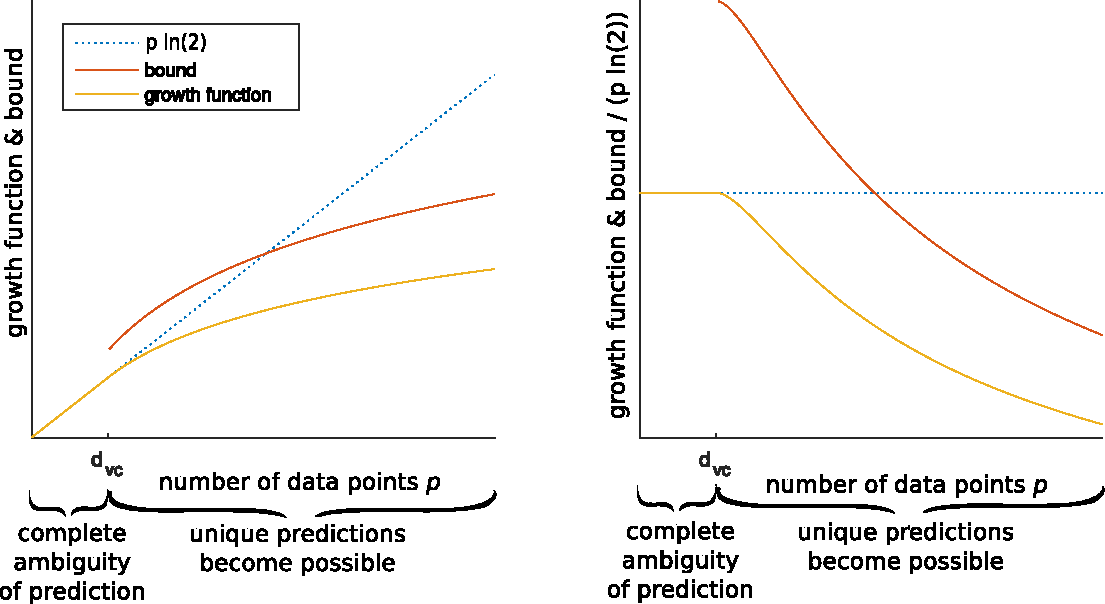
\includegraphics[height=5.7cm]{img/growth_function_clean}
	\end{center}
	\vspace{-2mm}
	$d_{VC}$: capacity measure of the model class\\
	small $d_{VC}$: small sample size sufficient for learning\\
	large $d_{VC}$: large sample size required

		%\item growth function defines VC-dimension $\dvc$
		%\item higher capacity $\rightarrow$ more different labelings
\end{frame}



\subsection{Revisit convergence of ERM}
\mode<article>{
\begin{frame}\frametitle{\subsecname}\label{sec:convergence_erm_revisit}
			
			Convergence of Empirical risk minimization is guaranteed:
			
			For a model class with \emph{finite} $\dvc$\notesonly{, the empirical training error will converge to the generalization error
			with more data. That is:}
			\begin{equation}
				\lim_{p \to \infty}
						E^T_{[\vec w]} = E^G_{[\vec w]}
			\end{equation}
			
			The requirement is that $\dvc$ is \emph{finite}.
			
			\mode<article>{The training error converges to the generalization error.
			}
			In terms of risk, this would be:
			
			\begin{equation}
				\lim_{p \to \infty} 
					R_{\text{emp}[\vec w]} = R_{[\vec w]}
			\end{equation}
			
			\begin{equation}
				\lim_{p \to \infty} P\bigg\{ 
					{
						\Big|R_{(\vec w_p)} - R_{(\vec w_0)}\Big| 
					}
				\geq \eta \bigg\}\;\;=\;\; 0 \,, \quad \forall \eta > 0
				\label{eq:risktozero}
			\end{equation}
			
			\textbf{But} Our dataset is never going to be infinitely large. Therefore, a more realistic formulation would be that ERM converges to some small $\epsilon$.\\
			We therefore reiterate \eqref{eq:convergenceeps}:
			
			\begin{equation}
				\lim_{p \to \infty} P\bigg\{ 
					{
						\Big|R_{(\vec w_p)} - R_{(\vec w_0)}\Big| 
					}
				\geq \eta \bigg\}\;\;<\;\; \epsilon \,, \quad \forall \eta > 0
				\label{eq:risktozero}
			\end{equation}
			
			The takeaway from the growth function and the bounds is that it defines the value of $\eta$ in \eqref{eq:convergenceeps} that can be targeted when training a specific model with a finite set of $p$ points.
			
			
\end{frame}
}

%TODO
%We replace  
%η
  %by this juggernaut term. We don't ask you to reproduce it. The important thing is to understand what happens when you select a larger value for p. The bound becomes tighter. This should not come as a surprise. In #30 we had the case of p approaching infinity which allowed us to bound everything by some constant  
%η
 %. Slide #31 expands this constant into terms that are a function of p. The bound has to be sensitive to p. #31 does not add new information but only rearranges the terms to being back  
%η
  %and express the confidence in terms of the size of the data set instead of  
%ϵ
 %.
 


\begin{frame}\frametitle{The solution to learning problem 2} 
	\begin{center}
		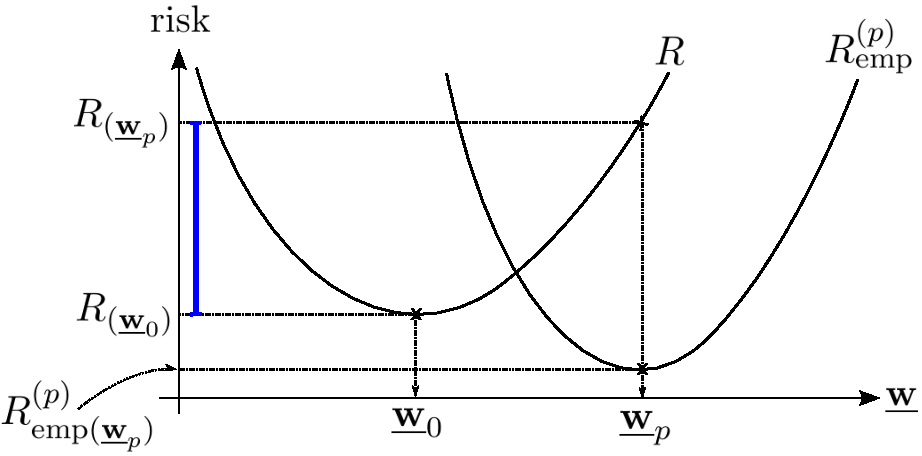
\includegraphics[width=9cm]{img/section2_fig1_question1}
	\end{center}
	\begin{enumerate}\setcounter{enumi}{1}
		\item \textbf{finite samples:} deviation from the optimal model
			\vspace{-2mm}
			\begin{equation}
				P\bigg\{ {%\color{question1} 
				\Big| R_{(\vec w_p)} - R_{(\vec w_0)} \Big| }
					> \Big(\smallfrac{G^\Lambda_{(2p)} 
						- \ln \frac{\epsilon}{8}}{p} \Big)^\frac{1}{2}
					+ \Big(-\smallfrac{\ln \frac{\epsilon}{2}}{2p} 
						\Big)^\frac{1}{2} + \smallfrac{1}{p}
				\bigg\} < \epsilon
					\label{eq:boundgenerlizationdeviation}
			\end{equation}
			\vspace{-4mm}
			\iitem{ finite $\dvc$: increased sample size $p$ 
				$\Rightarrow$ reduction of the bound}
	\end{enumerate}
\end{frame}

\mode<presentation>{
\begin{frame}\frametitle{Re-thinking $\eta$: bounded by the growth function}
\begin{center}
	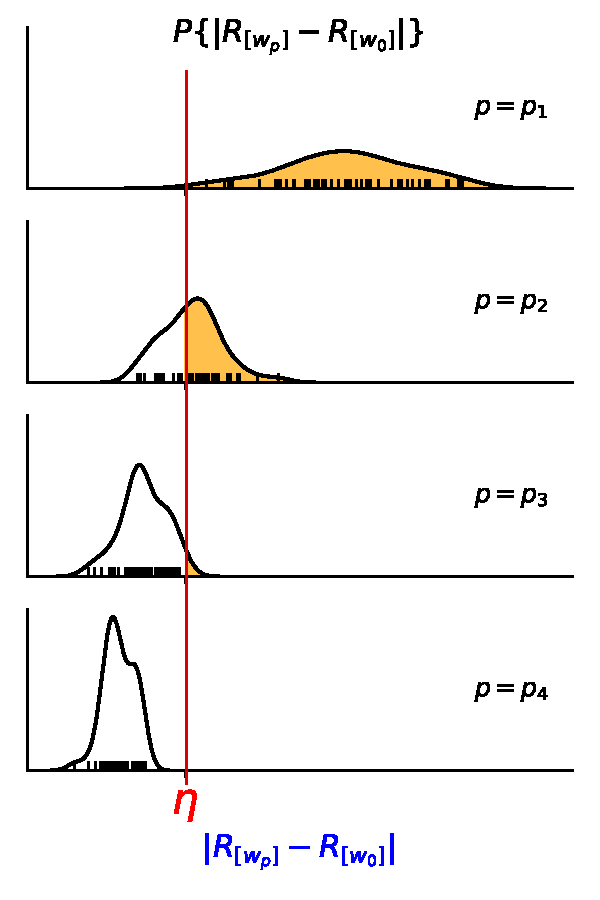
\includegraphics[height=6cm]{img/PdeltaReta}
\end{center}
			\begin{equation}
				\lim_{p \to \infty} P\bigg\{ 
					{
						\Big|R_{(\vec w_p)} - R_{(\vec w_0)}\Big| 
					}
				\geq \eta \bigg\}\;\;<\;\; \epsilon \,, \quad \forall \eta > 0
				\label{eq:risktozero}
			\end{equation}
\end{frame}
}

\mode<article>{
Recall that we were using \figref{fig:PdeltaReta} to see how the probability of scoring non-zero training error vanishes with more data points.
More data is good and the distribution of errors shifts to the left of $\eta$. While doing so, we were treating $\eta$ as a constant.

After learning about the growth function, we discover that $\eta$ is not necessarily an arbitrary constant but a value that is tied to the growth function of the model class \underline{and} the number of training points $p$\footnote{If interested, the supplementary material derives the relationship between $\eta$, the growth function and $p$}. Knowing that this relationship exists we learn that the vertical line we drew at $\eta$ is capable of shifting as a result of varying $p$ and the growth function.

Increasing $p$ not only causes the distribution to shift to the left but also
causes $\eta$ to shift to the left. Both will not necessarily shift at the same rate but
it just means that increasing $p$ no longer guarantees probability of
zero. The bound gets \textit{lower} with larger $p$. Why should we not be surprised by
this? One word: underfitting. Increasing $p$ and not getting rid of error is
indicative of a bias in our model class. It will not benefit from throwing
more data at it.

A larger growth function shifts the $\eta$ line to the right. The
distribution shifts to the right, so both are moving away from each other. The
probability of error vanishes and we get zero error on the training set. It's important to remember that the zero
error will only occur on the training set. Forgetting about it will make us
think choosing a larger growth function will always make us generalize
better and this is simply not the case. This is why we need to bound the probability by the
generalization capabilities of the model class which leads us to the following formulation:
}

\begin{frame}\frametitle{The solution to learning problem 3} 
	\begin{center}
		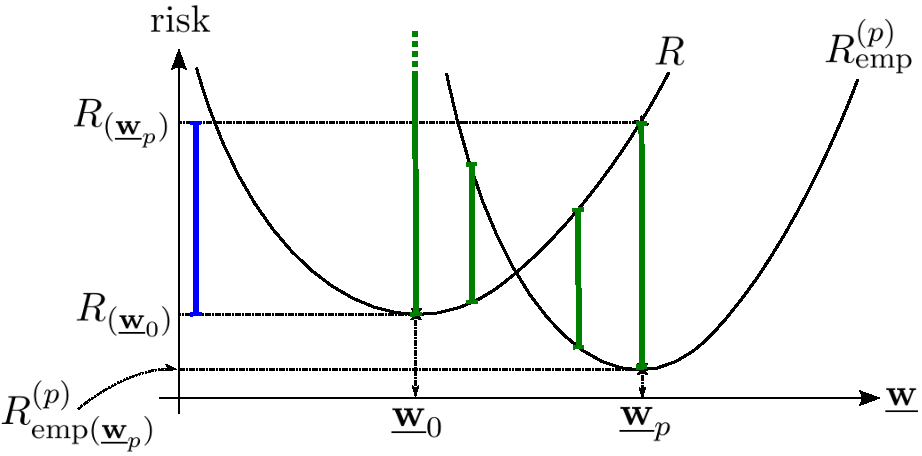
\includegraphics[width=9cm]{img/section2_fig1_question2_lessw}
	\end{center}
	\begin{enumerate}\setcounter{enumi}{2}
		\item \textbf{finite samples:} bound on the generalization error
			\vspace{-2mm}
			\begin{equation}
				P\bigg\{ \sup\limits_{\vec w \in \Lambda}
					{%\color{question2} 
						\Big|R_{(\vec w)} - R^{(p)}_{\text{emp}(\vec w)}\Big| 
					} > \eta
				\bigg\} < 4 \exp\Big( G^\Lambda_{(2p)} 
					- p \big( \eta - \smallfrac{1}{p} \big)^2 \Big)
					\label{eq:boundgenerlization}
			\end{equation}
			\vspace{-4mm}
			\iitem{ bound non-trivial only if $G^\Lambda_{(2p)}$ 
				is sub-linear in $p$}
	\end{enumerate}
\end{frame}

\mode*

\clearpage

\mode<all>
\section{Results statistical learning theory}

\begin{frame}\frametitle{Results of Statistical Learning Theory}
		\begin{itemize}
			\item formulation of conditions under which ERM works and its convergence \notesonly{(cf. \sectionref{sec:convergence_erm})}
			\item bounds describing \textbf{generalization ability} of ERM \\
            
            For a finite training set, the generalization error is bound with probability $1-\epsilon$:
            \begin{equation}
				E^{G}_{[\vec w]} \;\le\; E^{T}_{[\vec w]} + \sqrt{\frac{\dvc \left(\ln \frac{2\,p}{\dvc} + 1\right)-\ln\frac{\epsilon}{4}}{p}} +\frac{1}{p} \quad \text{for } p > \dvc
				\label{eq:generalizationresults}
            \end{equation}
            
            \mode<article>{
            where $\dvc \left(\ln \frac{2\,p}{\dvc} + 1\right) =: G^{\Lambda}_{(2p)}$ from \eqref{eq:growthpiecewise} for $p > \dvc$.
            }
            
            \mode<article>{
            \eqref{eq:generalizationresults} is obtained by solving \eqref{eq:boundgenerlization} for $\epsilon$ \footnote{If interested, cf. supplementary material ``Deviations from the optimal model''}.
            }
            
            100\% overfitting for $p\,<\,\dvc$.
            
            Bound allows calculating $p$ to target a given generalization error.
            
			\item inductive inference for \textbf{small sample size}s 
				based on these bounds
			\item methods for implementing this new type 
				of inference ($\rightarrow$ maximum margin classifiers e.g. {SVMs})
		\end{itemize}
\end{frame}

\mode*

\clearpage

\section{References}
\begin{frame}[allowframebreaks] \frametitle{References}
	%\footnotesize
	\scriptsize
	\bibliographystyle{plainnat}
	\bibliography{bibliography}
\end{frame}

\end{rightcolumn}
\end{paracol}

\end{document}
